\documentclass{article}
\usepackage{graphicx} % Extended graphics inclusions
\usepackage{float}
\usepackage{url} % For \url{}
\usepackage{../config/atxy} % For front cover
\usepackage{amsfonts} % Needed for some fonts
\usepackage[usenames]{color} % Needed for colored R input/output
\usepackage{pdfcolmk} % Correct some problems with the color stack


\title{RISA \textit{in silico} with seqinR}
\author{Lobry, J.R.}

\usepackage{/Library/Frameworks/R.framework/Resources/share/texmf/Sweave}
\begin{document}
%
% To change the R input/output style:
%
\definecolor{Soutput}{rgb}{0,0,0.56}
\definecolor{Sinput}{rgb}{0.56,0,0}
\DefineVerbatimEnvironment{Sinput}{Verbatim}
{formatcom={\color{Sinput}},fontsize=\footnotesize, baselinestretch=0.75}
\DefineVerbatimEnvironment{Soutput}{Verbatim}
{formatcom={\color{Soutput}},fontsize=\footnotesize, baselinestretch=0.75}
%
% This removes the extra spacing after code and output chunks in Sweave,
% but keeps the spacing around the whole block.
%
\fvset{listparameters={\setlength{\topsep}{0pt}}}
\renewenvironment{Schunk}{\vspace{\topsep}}{\vspace{\topsep}}
%
% Rlogo
%
\newcommand{\Rlogo}{\protect
\includegraphics[height=1.8ex,keepaspectratio]{../figs/Rlogo.pdf}}
%
% Shortcut for seqinR:
%
\newcommand{\seqinr}{\texttt{seqin\bf{R}}}
\newcommand{\Seqinr}{\texttt{Seqin\bf{R}}}
\fvset{fontsize= \scriptsize}
%
% R output options and libraries to be loaded.
%
%
%  Sweave Options
%
% Put all figures in the fig folder and start the name with current file name.
% Do not produce EPS files
%


\maketitle
\tableofcontents
% BEGIN - DO NOT REMOVE THIS LINE

\section{Introduction}

By RISA we mean here Ribosomal Intergenic Spacer Analysis. Ribosomal
genes are highly conserved so that it is relatively easy to design
universal PCR primers. On the other hand the intergenic space is under
weaker selective pressure, yielding more between species variability
in terms of length.

Making a RISA \textit{in silico} is an interesting task for seqinR :
we want to extract ribosomal genes from general databases and then
to compute the fragment length between the two primers.

\section{The primers}

Let's use the following primer in the 16S, also known as 
S-D-Bact-1522-b-S-20 \cite{RanjardL2000}:

\begin{Schunk}
\begin{Sinput}
 library(seqinr)
 (amo1 <- tolower("TGCGGCTGGATCCCCTCCTT"))
\end{Sinput}
\begin{Soutput}
[1] "tgcggctggatcccctcctt"
\end{Soutput}
\end{Schunk}


Let's use the following primer in the 23S, also known as 
L-D-Bact-132-a-A-18 \cite{RanjardL2000}:

\begin{Schunk}
\begin{Sinput}
 (amo2 <- tolower("CCGGGTTTCCCCATTCGG"))
\end{Sinput}
\begin{Soutput}
[1] "ccgggtttccccattcgg"
\end{Soutput}
\end{Schunk}

We work thereafter with its complementary sequence as follows:

\begin{Schunk}
\begin{Sinput}
 cplt <- function(x) c2s(comp(rev(s2c(x))))
 (amo2 <- cplt(amo2))
\end{Sinput}
\begin{Soutput}
[1] "ccgaatggggaaacccgg"
\end{Soutput}
\end{Schunk}

\section{Finding a primer location}

We want to fing a substring allowing for mismatches (say 3)
but no indels\footnote{It would be better to code this as
a regular expression to use standard tools but I don't know how 
to do this.}. Let's
write a function for this. Here we just use a moving window to count the
number of matches for all positions and return the one with the
maximum value. If the maximum number of matches if not enough, \texttt{NA}
is returned instead. In the verbose the function produces a plot
to check that everything is OK.

\begin{Schunk}
\begin{Sinput}
 find.amo <- function(amo, myseq, verbose = FALSE, nmiss = 3) {
     y <- numeric(nchar(myseq))
     myseq2 <- s2c(myseq)
     for (k in seq_len(nchar(myseq) - nchar(amo))) {
         y[k] <- sum(s2c(amo) == myseq2[k:(k + nchar(amo) - 
             1)])
     }
     if (verbose) 
         plot(1:nchar(myseq), y, type = "h", ylim = c(0, nchar(amo)), 
             main = amo)
     nmismatch <- nchar(amo) - max(y)
     if (verbose) 
         print(paste(nmismatch, "mismatch"))
     if (nmismatch > nmiss) {
         warning(paste("too many mismatches:", nmismatch))
         return(NA)
     }
     if (verbose) 
         rug(which.max(y), col = "red")
     return(which.max(y))
 }
\end{Sinput}
\end{Schunk}

Example with a random sequence:

\begin{Schunk}
\begin{Sinput}
 rseq <- c2s(sample(s2c("acgt"), 500, rep = T))
 find.amo(amo1, rseq, verbose = TRUE)
\end{Sinput}
\begin{Soutput}
[1] "9 mismatch"
[1] NA
\end{Soutput}
\end{Schunk}
\includegraphics{../figs/risa-essai}

Now insert a perfect target for the first primer at position 100 in this random sequence
to check that everything is OK :

\begin{Schunk}
\begin{Sinput}
 substr(rseq, 100, 100 + nchar(amo1)) <- amo1
 find.amo(amo1, rseq, verb = T)
\end{Sinput}
\begin{Soutput}
[1] "0 mismatch"
[1] 100
\end{Soutput}
\end{Schunk}
\includegraphics{../figs/risa-essai2}

\section{Compute the length of the intergenic space}

More exactly we want to compute the length of the fragment amplified
between two PCR primers. Here it is, note that we have to take into account
whether the primers are on the direct or complementary strand and the
length of the primers:

\begin{Schunk}
\begin{Sinput}
 risa.length <- function(myseq, amo1, amo2, forward, verbose = FALSE) {
     if (forward) {
         posamo1 <- find.amo(amo1, myseq, verbose = verbose)
         posamo2 <- find.amo(amo2, myseq, verbose = verbose)
     }
     else {
         posamo1 <- find.amo(cplt(amo1), myseq, verbose = verbose)
         posamo2 <- find.amo(cplt(amo2), myseq, verbose = verbose)
     }
     if (is.na(posamo1)) 
         return(list(res = NA, posamo1 = NA, posamo2 = NA))
     if (is.na(posamo2)) 
         return(list(res = NA, posamo1 = NA, posamo2 = NA))
     return(list(res = abs(posamo2 - posamo1) + ifelse(forward, 
         nchar(amo2), nchar(amo1)), posamo1 = posamo1, posamo2 = posamo2))
 }
\end{Sinput}
\end{Schunk}

Let's check this with an artificial example by inserting the second primer at
position 300 in our random sequence:

\begin{Schunk}
\begin{Sinput}
 nchar(amo2)
\end{Sinput}
\begin{Soutput}
[1] 18
\end{Soutput}
\begin{Sinput}
 substr(rseq, 300, 300 + nchar(amo2)) <- amo2
 risa.length(rseq, amo1, amo2, forward = T)$res
\end{Sinput}
\begin{Soutput}
[1] 218
\end{Soutput}
\begin{Sinput}
 risa.length(cplt(rseq), amo1, amo2, forward = F)$res
\end{Sinput}
\begin{Soutput}
[1] 218
\end{Soutput}
\end{Schunk}

Looks OK for me.

\section{Compute IGS for a sequence fragment}

\begin{figure}
\centering
\fbox{
\begin{minipage}{\textwidth}
\centering
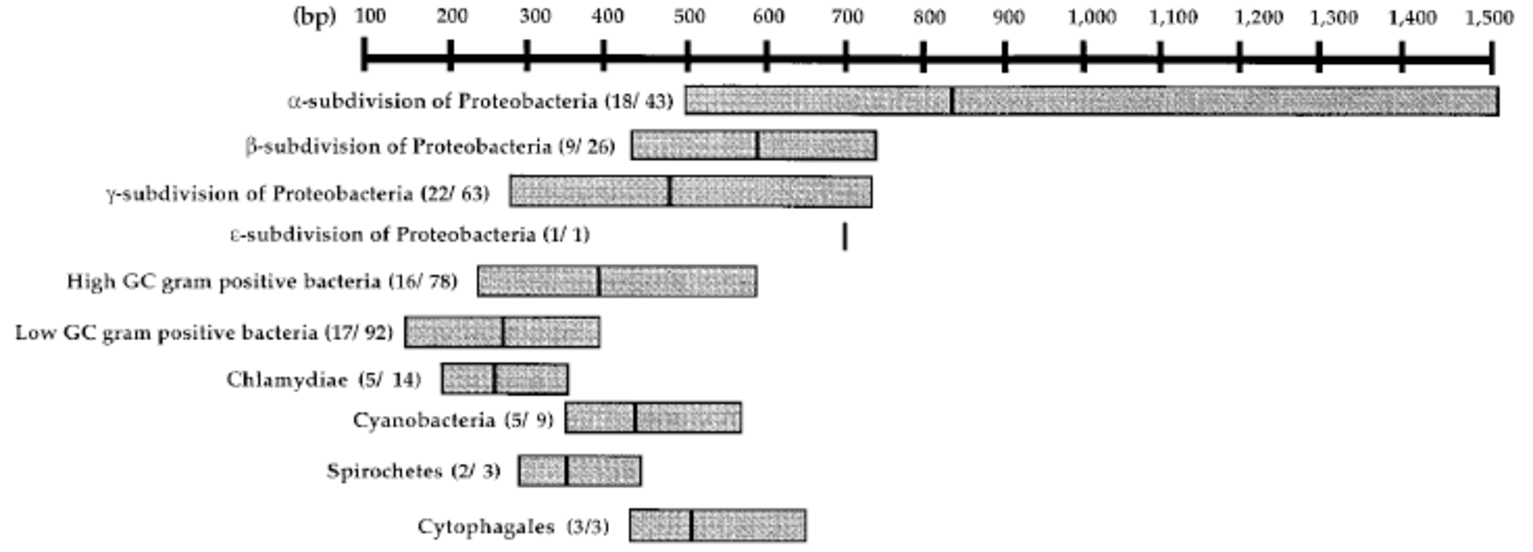
\includegraphics[width=\textwidth]{../figs/fig1RanjardL2000}
\caption{Screenshot of a part of figure 1 in \cite{RanjardL2000} showing the observed range
of ribosomal intergenic space length in bacterial species (n = 428).}
\label{fig1RanjardL2000}
\end{minipage}
}
\end{figure}


By sequence fragment we mean here a genbank entry accessed
by its name (\texttt{mnemo} in the code thereafter).
There could be more than one rRNA operon in the sequence fragment
but there should be the same number of 16S and 23S genes.
There is a maximum length to the 16S-23S segemnt to avoid problems when genes are
not annotated in consecutive order, in this case \texttt{NA}
is returned. The default maximum length of 10 kb is conservative,
the maximum observed value is 1.5 kb (\textit{cf} Fig. \ref{fig1RanjardL2000}),
some post-processing of the results is most likely necessary to remove outliers.
In case of problem during the query process the value \texttt{-Inf} is
returned to denote this.

\begin{Schunk}
\begin{Sinput}
 mn2risa <- function(mnemo, amo1, amo2, maxlength = 10000, verbose = FALSE){
   if(verbose) print(paste("mn2risa -->", mnemo))
   #
   # Make a list on server with the requested entry name:
   #
   try.res <- try(query("frag", paste("N=", mnemo)))
   if(inherits(try.res, "try-error")) return(-Inf)
   #
   # From this make a list with all subsequences that are rRRA genes
   # with a keyword containing 16S anywhere in it:
   #
   try.res <- try(query("frag16S", "frag ET T=RRNA ET K=@16S@"))
   if(inherits(try.res, "try-error")) return(-Inf)
   if(verbose) print(paste("n 16S = ", frag16S$nelem))
   #
   # The same but with 23S anywhere in keywords:
   #
   try.res <- query("frag23S", "frag ET T=RRNA ET K=@23S@")
   if(verbose) print(paste("n 23S = ", frag23S$nelem))
   if(inherits(try.res, "try-error")) return(-Inf)
   #
   # We want the same number of 16S and 23S rRNA in the entry:
   #
   if(frag16S$nelem != frag23S$nelem) return(NA)
   #
   # We retrieve the location of all 16S and 23S rRNA in this genbank entry:
   #
   try.res <- try(loc16S <- getLocation(frag16S))
   if(inherits(try.res, "try-error")) return(-Inf)
   try.res <- try(loc23S <- getLocation(frag23S))
   if(inherits(try.res, "try-error")) return(-Inf)
   #
   # The result is a vector with as many elements as rRNA operons
   #
   n <- frag16S$nelem
   risa <- numeric(n)
   #
   # We loop now over all operons:
   #
   for(i in seq_len(n)){
     coord.16S <- loc16S[[i]]
     coord.23S <- loc23S[[i]]
     #
     # Test if the genes are in the forward or reverse strand:
     #
     if(coord.16S[1] < coord.23S[1]){
       forward <- TRUE
       if(verbose) print("forward")
     } else {
       forward <- FALSE	
       if(verbose) print("bacward")
     }
     if(verbose) print(paste("16S at", coord.16S[1], coord.16S[2], "23S at", coord.23S[1], coord.23S[2]))
     #
     # Check that our operon is not too long:
     #
     xmin <- min(coord.16S, coord.23S)
     xmax <- max(coord.16S, coord.23S)
     if(xmax - xmin > maxlength){
       warning(paste("Operon too long found, NA returned", mnemo, i))
       risa[i] <- NA
       next
     }
     #
     # Get just the sequence of the operon from the genbank entry. This
     # is the only place where we are retrieving sequence data. This
     # return an objet of class SeqFrag that we cast into a simple
     # character string.
     #
     try.res <- try(myseq <- as.character(getFrag(frag$req[[1]], xmin, xmax)))
     if(inherits(try.res, "try-error")){
       risa[i] <- -Inf
       next
     }
     if(verbose) print(paste("nchar myseq = ", nchar(myseq)))
     #
     # Compute the IGS length on this operon
     #
     risa[i] <- risa.length(myseq, amo1, amo2, forward, verbose = F)$res
   }
   return(risa)    
 }
\end{Sinput}
\end{Schunk}

Example with a fragment with one 16S and two 23S genes,
\texttt{NA} is returned as expected :

\begin{Schunk}
\begin{Sinput}
 mn2risa("BBRNAOPR", amo1, amo2, verb = T)
\end{Sinput}
\end{Schunk}

Example with a fragment with seven 16S and seven 23S genes,
the seven IGS lengths are returned :

\begin{Schunk}
\begin{Sinput}
 mn2risa("AE005174", amo1, amo2, verb = T)
\end{Sinput}
\end{Schunk}

\section{Compute IGS for a species}

We could work in fact at any taxonomical level, but suppose here that
we are interested by the species level. All we have to do is to find
the list of fragment where there is at least one 16S and one 23S gene.
We use here all the power of ACNUC query language. 


\begin{Schunk}
\begin{Sinput}
 sp2risa <- function(sp, amo1, amo2, verbose = TRUE){
   if(verbose) print(paste("sp2risa -->", sp))
   #
   # protect query with quotes, get all sequences attached the specie
   #  
   try.res <- try(query("cursp", paste("\"sp=", sp, "\"", sep=""), virtual=TRUE))
   if(inherits(try.res, "try-error")) return(-Inf)
   #
   # Get all 16S rRNA genes:
   #
   try.res <- try(query("res1", "cursp ET T=RRNA ET K=@16S@", virtual=TRUE))
   if(inherits(try.res, "try-error")) return(-Inf)
   #
   # Replace by mother sequences:
   #
   try.res <- try(query("res1", "ME res1", virtual=TRUE))
   if(inherits(try.res, "try-error")) return(-Inf)
   #
   # Get all 23S rRNA genes:
   #
   try.res <- try(query("res2","cursp ET T=RRNA ET K=@23S@", virtual=TRUE))
   if(inherits(try.res, "try-error")) return(-Inf)
   #
   # Replace by mother sequences:
   #
   try.res <- try(query("res2","ME res2",virtual=TRUE))
   if(inherits(try.res, "try-error")) return(-Inf)
   #
   # Keep only sequences that contains at least one 16S and 23S:
   #
   try.res <- try(query("res3", "res1 ET res2"))
   if(inherits(try.res, "try-error")) return(-Inf)
 
   if(verbose) print(paste("number of mother sequences = ", res3$nelem))
   seqnames <- getName(res3)
   result <- vector("list", res3$nelem)
   names(result) <- seqnames
   #
   # Loop over all sequences:
   #
   for(i in seq_len(res3$nelem)){
     try.res <- try(result[[i]] <- mn2risa(seqnames[i], amo1, amo2, verbose = verbose))
     if(inherits(try.res, "try-error")) result[[i]] <- -Inf
   }
   return(result)
 }
\end{Sinput}
\end{Schunk}


\section{Loop over many species}

\subsection{Preprocessing: select interesting species}

We select bacterial species for which there is at least one
entry with at least one 16S and one 23S gene:

\begin{Schunk}
\begin{Sinput}
 #
 # Choose a bank:
 #
 choosebank("genbank")
 #
 # Select all bacterial sequences with 23S:
 #
 query("allbact", "SP=bacteria ET T=RRNA ET K=@23S@", virtual = TRUE)
 #
 # Replace by mother sequences:
 #
 query("allbact", "ME allbact", virtual = TRUE)
 #
 # Look for 16S in them:
 #
 query("allbact", "allbact ET T=RRNA ET K=@16S@", virtual = TRUE)
 #
 # Get species names:
 #
 query("splist", "PS allbact")
 #
 # Save them into a file:
 #
 splist <- getName(splist)
 head(splist)
 length(splist)
 save(splist, file = "splist.RData")
\end{Sinput}
\end{Schunk}

\subsection{Loop over our specie list}

We loop now over our specie list. As this is long, we run
it overnight in batch, saving results on the fly to spy them.
When the species name is a single word this is most likely a genus,
then to avoid redundancy in computation with the underlying species,
it is not considered and a \texttt{+Inf} value is set. An empty list
means that no fragment with both 16S and 23S genes were found. A
missing value \texttt{NA} means that the PCR primers were not found.
A \texttt{-Inf} value means a problem while querying the server.

\begin{Schunk}
\begin{Sinput}
 load("splist.RData")
 resultat <- vector("list", length(splist))
 names(resultat) <- splist
 i <- 1
 for (sp in splist) {
     print(paste("===>", sp))
     if (length(unlist(strsplit(sp, split = " "))) == 1) {
         resultat[[i]] <- +Inf
         i <- i + 1
         next
     }
     try.res <- try(resultat[[i]] <- sp2risa(sp = sp, amo1, 
         amo2, verbose = TRUE))
     if (inherits(try.res, "try-error")) 
         resultat[[i]] <- -Inf
     save(resultat, file = "resultat.RData")
     print(paste("=>", resultat[[i]]))
     i <- i + 1
 }
\end{Sinput}
\end{Schunk}

\section{Playing with results}

\begin{Schunk}
\begin{Sinput}
 load("resultat.RData")
\end{Sinput}
\end{Schunk}

There shouldn't be any null entries in results, except if we are
spying them.

\begin{Schunk}
\begin{Sinput}
 lesnull <- (unlist(lapply(resultat, is.null)))
 (nnull <- sum(lesnull))
\end{Sinput}
\begin{Soutput}
[1] 1
\end{Soutput}
\begin{Sinput}
 resultat <- resultat[!lesnull]
\end{Sinput}
\end{Schunk}

Show how many fragments we have by species :

\begin{Schunk}
\begin{Sinput}
 table(unlist(lapply(resultat, length)))
\end{Sinput}
\begin{Soutput}
   1    2    3    4    5    6    7    8    9   10   11   12   13   14   15 
1567  253  114   51   24   22   27   11   10    6    6    3    2    6    5 
  16   17   18   19   20   21   22   23   24   25   26   29   31   35   37 
   4    3    6    1    4    1    5    1    2    1    3    2    1    1    1 
  39   45   64   69   71   72   80  107  139 
   1    1    1    1    1    1    1    1    1 
\end{Soutput}
\end{Schunk}

Show how many IGS of different size we have per species.

\begin{Schunk}
\begin{Sinput}
 igsdbysp <- unlist(lapply(resultat, function(x) length(unique(unlist(x)))))
 plot(table(igsdbysp), xlab = "Number of IGS of different size", 
     ylab = "Number of species")
\end{Sinput}
\end{Schunk}
\includegraphics{../figs/risa-ndIGSpsp}

Which are the species with the most important number of IGS?

\begin{Schunk}
\begin{Sinput}
 tail(igsdbysp[order(igsdbysp)], n = 30)
\end{Sinput}
\begin{Soutput}
           KLEBSIELLA PNEUMONIAE 342                 CAMPYLOBACTER JEJUNI 
                                   6                                    7 
                  PSEUDOMONAS PUTIDA         SHEWANELLA WOODYI ATCC 51908 
                                   7                                    7 
        SHEWANELLA SEDIMINIS HAW-EB3              ESCHERICHIA COLI CFT073 
                                   7                                    7 
                     VIBRIO CHOLERAE                    VIBRIO VULNIFICUS 
                                   7                                    7 
VIBRIO PARAHAEMOLYTICUS RIMD 2210633            BACILLUS HALODURANS C-125 
                                   7                                    7 
   HELIOBACTERIUM MODESTICALDUM ICE1                  CUPRIAVIDUS NECATOR 
                                   7                                    8 
             PSEUDOMONAS FLUORESCENS  CANDIDATUS COMPETIBACTER PHOSPHATIS 
                                   8                                    8 
             VIBRIO PARAHAEMOLYTICUS                  BACILLUS HALODURANS 
                                   8                                    8 
   ALKALIPHILUS METALLIREDIGENS QYMF                 SORANGIUM CELLULOSUM 
                                   8                                    9 
            BRADYRHIZOBIUM JAPONICUM           PSYCHROMONAS INGRAHAMII 37 
                                   9                                    9 
     GEOBACILLUS KAUSTOPHILUS HTA426           RHODOPSEUDOMONAS PALUSTRIS 
                                   9                                   10 
                    ESCHERICHIA COLI             GEOBACILLUS KAUSTOPHILUS 
                                  10                                   10 
               VIBRIO FISCHERI ES114                KLEBSIELLA PNEUMONIAE 
                                  11                                   12 
        PHOTOBACTERIUM PROFUNDUM SS9                      BACILLUS CEREUS 
                                  12                                   13 
               STAPHYLOCOCCUS AUREUS         UNCULTURED SYNECHOCOCCUS SP. 
                                  24                                   29 
\end{Soutput}
\end{Schunk}

How many IGS do we have there:

\begin{Schunk}
\begin{Sinput}
 brut <- unlist(resultat)
 length(brut)
\end{Sinput}
\begin{Soutput}
[1] 7659
\end{Soutput}
\begin{Sinput}
 brut2 <- brut[!is.na(brut)]
 length(brut2)
\end{Sinput}
\begin{Soutput}
[1] 4373
\end{Soutput}
\end{Schunk}

\begin{Schunk}
\begin{Sinput}
 tab <- table(brut2)
 x <- as.numeric(unlist(dimnames(tab)))
 y <- tab
 plot(x, y, type = "h", ylim = c(0, max(y)), main = "Global distribution of IGS length", 
     las = 1, ylab = "Count", xlab = "Size in bp", xlim = c(0, 
         1500))
 dst <- density(brut2, adj = 0.2)
 lines(dst$x, dst$y * max(y)/max(dst$y), col = "red", xpd = NA)
\end{Sinput}
\end{Schunk}
\includegraphics{../figs/risa-bplot}


\section*{Session Informations}

This part was compiled under the following \Rlogo{}~environment:

\begin{itemize}
  \item R version 2.7.2 (2008-08-25), \verb|i386-apple-darwin8.8.2|
  \item Locale: \verb|fr_FR.UTF-8/fr_FR.UTF-8/fr_FR.UTF-8/C/C/C|
  \item Base packages: base, datasets, grDevices, graphics, methods,
    stats, utils
  \item Other packages: MASS~7.2-44, ade4~1.4-9, ape~2.2-1,
    nlme~3.1-89, quadprog~1.4-11, seqinr~2.0-0, tseries~0.10-16,
    xtable~1.5-3, zoo~1.5-4
  \item Loaded via a namespace (and not attached): grid~2.7.2,
    lattice~0.17-13
\end{itemize}
There were two compilation steps:

\begin{itemize}
  \item \Rlogo{} compilation time was: Thu Oct 16 11:18:43 2008
  \item \LaTeX{} compilation time was: \today
\end{itemize}

% END - DO NOT REMOVE THIS LINE

%%%%%%%%%%%%  BIBLIOGRAPHY %%%%%%%%%%%%%%%%%
\clearpage
\addcontentsline{toc}{section}{References}
\bibliographystyle{plain}
\bibliography{../config/book}
\end{document}
